\chapter{Validating 126 million MARC records}

%\begin{abstract}
The paper describes the method and results of validation of 14 library catalogues. The format of the catalog record is Machine Readable Catalog (MARC21) which is the most popular metadata standards for describing books. The research investigates the structural features of the record and as a result finds and classifies different commonly found issues. The most frequent issue types are usage of undocumented schema elements, then improper values in places where a value should be taken from a dictionary, or should match to other strict requirements.
%\end{abstract}

%\keywords{metadata quality measurement, MARC21, Java, Big Data, Data Science}

\section{Introduction}
How should a book be described properly? This question has a long past (and an even longer future) with several proposed methods which evolved over time. In the current epoch in the history of cataloging or in other words bibliographic control we see the end of a period, and the start of a new one. There are different conflicting proposals on the table regarding what should be the new big thing, but there is a consensus on that from the middle of 60-es up until now the dominant record format of the book descriptions was MARC, MAchine Readable Cataloging developed and maintained by the Library of Congress \cite{marc21}. MARC is a format and also a semantic specification. It was invented -- after an investigative period started at the end of 1950s -- at the middle of the 1960s (at the age of punch cards) in a collaborative effort of different American libraries, led by Henriette Avram.\footnote{See MARC's early history in \cite{avram1975}} At that time the available information storage space was much less than it is nowadays, so the information should be compressed, therefore one of the main technical features of MARC is that wherever a piece of information could be described by an element of a closed list of terms this path is chosen. The record contains abbreviated forms, while the standard describes the abbreviated terms in detail. It makes the human understanding of MARC difficult in its native form, but makes the machine readability and thus validation easy. Theoretically at least. The problem is that during the decades while the basic structure of MARC remained the same, MARC continued to grown into a giant standard, with a number of such small or big dictionaries (which sometimes are externally developed and maintained by other organizations, such as the content classification schemes). Roy Tennant, in his famous (infamous for some), manifesto-like article \cite{tennant2002} pictures the situation with a colourful sentence „There are only two kinds of people who believe themselves able to read a MARC record without referring to a stack of manuals: a handful of our top catalogers and those on serious drugs.” Most of the open source tools for handling MARC concentrate on the structure, and take less care about the semantics, maybe because it would require a huge effort to make the standard itself machine readable in order to make such a tool aware of the meaning of the abbreviations.

Closing into the end of the MARC life cycle, it would be the appropriate time to examine some of the catalogues published under open licenses, and check their quality. This paper examines 126 million\footnote{126 638 140 to be exact} MARC records from 16 different library organizations whether they match the structural requirements of the standard. In order to achieve this goal the author created an open source software application written in Java which implements the structural rules of the MARC21 Bibliographic Description as Java classes.\footnote{https://github.com/pkiraly/metadata-qa-marc} The rule set in a machine readable way could be exported in Avram specification conformant JSON format,\footnote{http://format.gbv.de/schema/avram/specification} so other tools could reuse it.

\section{Why it important to validate metadata?}

I would not claim that metadata plays the most important rule in using the digitized text or audiovisual media. The large text corpus is much more effective than metadata when it comes to searching. However there are some other fields where metadata is very useful. \cite{moreux2016} showed that a successful data mining approach on large corpora of digitized journals should use metadata as well. According to \cite{nanni2017} one of the current research topics in natural language processing is to reuse the contextual information provided by the metadata of the text. There are several examples when different digital humanities research uses metadata and full text together to reveal new facts (among others \cite{jockers2013}, \cite{smith2017} and \cite{lahti2019}). \cite{brown2016} calls attention to the effects of metadata biases: ``because researchers have to rely on metadata to organize and navigate large corpora, there may be a significant number of relevant but essentially `invisible’ documents.''. ``Collections as data''\footnote{https://collectionsasdata.github.io/} is a recent LAM movement, it aims to ``foster a strategic approach to developing, describing, providing access to, and encouraging reuse of collections that support computationally-driven research and teaching''.  Their statement sheds light to the importance of metadata: ``Trustworthy collections as data should include open, robust metadata'' \cite{santabarbarastatement2017}. They collect different use cases which includes services for researcher backed by metadata.

Library catalogues became widely reused. MARC is a well documented format, there are different open source and commercial tools to work with, some of the biggest catalogues are openly accessible and reusable, the records are meticulously curated and usually contain contextual information, all of these makes them easily usable data sources for different researches. The reuse aspect makes the effects of metadata issues bigger, since they not just break Ranganathan's rules\footnote{https://en.wikipedia.org/wiki/Five\_laws\_of\_library\_science}, but they effect scientific conclusions. This research is not looking for the ``perfect metadata'' \cite{bade2008}, but aims to reveal the improvable parts of catalogues.

\section{Introduction to MARC}

While this paper can not give a full encounter of MARC, it just provides the most important features, which helps in the understanding of the resulting quality measurement. 

An example record (excerpt):

\begin{small}
\begin{Verbatim}[samepage=true]
01136cnm a2200253ui 4500
001 002032820
005 20150224114135.0
008 031117s2003    gw            000 0 ger d
020   $a3805909810
100 1 $avon Staudinger, Julius,$d1836-1902
      $0(viaf)14846766
245 10$aJ. von Staudingers Kommentar zum ... /
      $cJ. von Staudinger.
250   $aNeubearb. 2003$bvon Jörn Eckert
260   $aBerlin :$bSellier-de Gruyter,$c2003.
300   $a534 p. ;.
500   $aCiteertitel: BGB.
500   $aBandtitel: Staudinger BGB.
700 1 $aEckert, Jörn
852 4 $xRE$bRE55$cRBIB$jRBIB.BUR 011 DE 021
      $p000000800147
\end{Verbatim}
\end{small}

The above example is a widely accepted representation of a MARC record however MARC is stored differently in MARC files. It has a semi-binary format, it uses some delimiter characters and fixed length fields to separate content parts. 

The first line is the leader (sometimes abbreviated as LDR), it is a fixed length field and a component of individual ``portions''. We should split the content this way (here `\texttt{|}' characters represent the boundaries between the portions, the first two lines denote character positions):

\begin{small}
\begin{Verbatim}[samepage=true]
0               1                2
01234 5 6 7 8 9 0 1 2345 6 7 8 9 0 1 2 3
01136|c|n|m| |a|2|2|0025|3|u|i| |4|5|0|0
\end{Verbatim}
\end{small}

Using the positions as the key, the meaning of the individual portions should be read as
\begin{itemize}
 \setlength{\parskip}{0pt}
 \setlength{\itemsep}{0pt plus 1pt}
 \item \texttt{LDR/0-4}: Record length. `01136’ -- is a number padding with zeros (max. value: 99999) denoting the length of the record, so this record is 1136 byte long. 
 \item \texttt{LDR/5}: Record status. `c’ is a dictionary term, means ``Corrected or revised''
 \item \texttt{LDR/6}: Type of record: `n’ is not among the defined types, this is an error
 \item \texttt{LDR/7}: Bibliographic level. `m’ means ``Monograph/Item''
 \item ...
\end{itemize}

In this document I will use the term `subfield' for these information (the standard does not have a term for this).

Different library materials require different descriptive element sets, however in MARC -- maybe due to the necessity of compressing information -- there is not a single ``record type'' field. Instead its value comes from the combination of two subfields of the Leader: the Type of Record, and the Bibliographic level (see Table \ref{table:record_type}). Several other elements of the schema depend on the value of this combination, however -- as we will see -- there are examples where the combination returns an undefined value.

\afterpage{%
 \clearpage% Flush earlier floats
    \thispagestyle{empty}% empty page style (?)
    \begin{landscape}% Landscape page
\begin{table}
  \caption{Record type}
  \label{table:record_type}
  \hspace{-2cm}
  \begin{minipage}{\textwidth}
  \begin{tabular}{lllllll}
    \toprule
    \multicolumn{2}{c}{Type of record (LDR/05)}&\multicolumn{2}{c}{Bibliographic level (LDR/06)}&type&\multicolumn{2}{c}{Form of material (006/00)}\\
    \midrule
    a&Language material&a&Monographic component part&Books&a&Language material\\
    &&c&Collection&\\
    &&d&Subunit&\\
    &&m&Monograph/Item&\\
    \midrule
    a&Language material&b&Serial component part&Continuing Resources&s&Serial/Integrating resource\\
    &&i&Integrating resource&\\
    &&s&Serial&\\
    \midrule
    t&Manuscript language material&&&Books&t&Manuscript language material\\
    \midrule
    c&Notated music&&&Music&c&Notated music\\
    d&Manuscript notated music&&&&d&Manuscript notated music\\
    i&Nonmusical sound recording&&&&i&Nonmusical sound recording\\
    j&Musical sound recording&&&&j&Musical sound recording\\
    \midrule
    e&Cartographic material&&&Maps&e&Cartographic material\\
    f&Manuscript cartographic&&&&f&Manuscript cartographic\\
    &material&&&&&material\\
    \midrule
    g&Projected medium&&&Visual Materials&g&Projected medium\\
    k&Two-dimensional&&&&k&Two-dimensional\\
    &nonprojectable graphic&&&&&nonprojectable graphic\\
    o&Kit&&&&o&Kit\\
    r&Three-dimensional artifact or&&&&r&Three-dimensional artifact or\\
    &naturally occurring object&&&&&naturally occurring object\\
    \midrule
    m&Computer file&&&Computer Files&m&Computer file/Electronic resource\\
    \midrule
    p&Mixed materials&&&Mixed Materials&p&Mixed materials\\
  \bottomrule
\end{tabular}
\end{minipage}
\end{table}
    \end{landscape}
    \clearpage% Flush page
}

Leader and fields 001-008 are so called control fields. Most of them are structurally similar to the Leader. The interpretation of 008 is dependent from the record type as defined by the combination mentioned above. Let's see the split of 008.

\begin{small}
\begin{Verbatim}[samepage=true]
0           1           2                3  
012345 6 7890 1234 567 8901 2 3 4567 8 9 0 1 2 3 4 567 8 9
031117 s 2003      gw                  0 0 0   0   ger   d
......|.|....|....|...|____|_|_|____|_|_|_|_|_|_|_|...|.|.
\end{Verbatim}
\end{small}

Here the first five (in position 0-17: different dates and place of publication) and the last three subfields (35-39: language, is the record modified?, cataloging source) are common for all types (denoted by dots), but the in-between part (18-34, denoted by underscores) are type-specific (for a book: illustrations, target audience, form of item, nature of contents, government publication, conference publication, Festschrift, index, literary form, biography -- all encoded) and does not only provide the meaning, but the internal structure as well (the number of portions and their positions)! This structure is quite fragile, one single character deletion from these fields would break the structure and mix the meaning of a position.

From 010 up until the end of the record are `datafields'. Their internal structure is different from that of the control fields. They have two indicators and one or more subfields. The indicators contain a single character to represent dictionary terms -- usually they are qualifiers of the subfields. The subfields start with a `\$' character, then comes a character long subfield code, and finally the value of the subfield. The value could be

\begin{itemize}
 \setlength{\parskip}{0pt}
 \setlength{\itemsep}{0pt plus 1pt}
 \item a code, or
 \item a literal value, which might be
 \begin{itemize}
  \setlength{\parskip}{0pt}
  \setlength{\itemsep}{0pt plus 1pt}
  \item a free text, or
  \item a dictionary term, or
  \item a string match to a fixed format (e.g. yymmdd), or
  \item a combination of fixed format string and dictionary terms (e.g. for 045's subfield `a' -- conventionally abbreviated as 045\$a in the string ``d7n6'' `d7' means B.C. 299-200, `n' means A.D. `900-999', and 6 stands for the 60-es of that century)\footnote{http://www.loc.gov/marc/bibliographic/bd045.html}, or
  \item combination of fixed positions and dictionary terms
 \end{itemize}
\end{itemize}

Both the field and the subfield can be repeatable or non-repeatable.

\subsection{The validation tool}

In order to validate MARC records I have developed a software. The core of the software is a data model, which records the whole MARC 21 Bibliographic documentation as a set of Java classes. In the model the main units are the fields (\emph{DataFieldDefinition} class), which have the code of the tag (such as 245), it's label (``Title Statement''), cardinality (repeatable or non repeatable), the URL of the definition at the Library of Congress page (\url{https://www.loc.gov/marc/bibliographic/bd245.html}). Then come the definition of the indicators, each having label, list of possible codes and their label. The last part of the field definition is the list of subfields: code, label, cardinality. The standard provides notes for obsolete elements, the Java class stores them as historical codes and subfields. Whenever it was possible I also recorded the BIBFRAME 2.0 equivalences based on the MARC 21 to BIBFRAME 2.0 Conversion Specifications\footnote{https://www.loc.gov/bibframe/mtbf/}. BIBFRAME names holds meaning (e.g. ``responsibilityStatement'' versus MARC's 245\$c, which is a language neutral notation) which could be uses in exporting data, because they don't contain spaces, so could be processed without problems in different software environments and self-describing. Since naturally there is no BIBFRAME equivalent for all MARC element, I have created a similar machine-readable tag. Some elements in MARC has a specially encoded value (e.g. the \$6 subfield in lots of field, which records linkage between parallel elements), so the model let us to attach content parsers. Several subfields should contain a term from a controlled dictionary and some of the subfields have formal rules to check whether they are valid or not. The tool contains all these dictionaries and validator classes have been implemented to check against these rules. Some rules are outside of MARC such as ISBN and ISSN rules. These identifiers are composite of a sequence of numbers, where the last one is a check digit, it should be equal of a result of a sequence of computations with all of the remaining numbers. It is also possible to connect external online tools to validate specific MARC element. I made some experiments with the automatic Universal Decimal Classification (UDC) analyser service developed by Attila Piros\footnote{\url{http://piros.udc-interpreter.hu/}}. The experience showed, that these kind of tools could be part of the validation process if they are fast enough, otherwise it is more advisable to extract data from the records (in this case the subfields containing UDC classification numbers) and run the UDC analysis asynchronously. As part of the FRBR works Tom Delsey created a mapping between the 12 functions and the MARC elements~\cite{delsey2003}. The Java model also built in this mapping.

The tool works together with another Java library, Marc4j\footnote{\url{https://github.com/marc4j/marc4j}}. With the help of this library my tool can read from binary MARC and from MARCXML formats. In regards to parallel processing with Apache Spark, the tool can read from a special MARC binary format where the records are separated with line breaks.\footnote{See details at \url{http://pkiraly.github.io/2018/01/18/marc21-in-spark/}.}

As a side effect, those knowledge built into the tool makes it useful for different other tasks, not just validation. One can use for formatting records, extracting information, index with Apache Solr, etc.

Since it took long time to build this model, I thought it would be useful to make it exportable, so other MARC related projects could use it as a machine-readable MARC specification. Jakob Voß introduced Avram JSON schema\footnote{\url{http://format.gbv.de/schema/avram/specification}} to provide a language for creation of machine readable metadata specification. Due to the implementation of this schema the tool can export MARC into Avram schema.  

\subsection{Addressing elements - MARCspec}

In the process of MARC validation it is important that we should be able to address specific parts of the record. For XML format this purpose is fulfilled by XPath, a W3C standard. For JSON there is not such a standard, but Stefan Gössner proposed JSONPath\footnote{http://goessner.net/articles/JsonPath/} for this purpose. We saw that \verb|245$a| is a conventional way to address subfield `a' of field 245, however for the less trivial uses cases (see them below) there are no similar conventions. Carsten Klee, the librarian of Zeitschriftendatenbank (Berlin) proposed MARCspec, a common MARC record path language\footnote{http://marcspec.github.io/MARCspec/marc-spec.html}, and that is what the tool implemented. Here are some MARCspec expressions:

\begin{itemize}
 \setlength{\parskip}{0pt}
 \setlength{\itemsep}{0pt plus 1pt}
  \item \verb|260| -- field
  \item \verb|245^2| -- the second indicator of a field
  \item \verb|700[0]| -- the first instance of a field
  \item \verb|245$c| -- a subfield
  \item \verb:245$b{007/0=\a|007/0=\t}: -- subfield ‘b’ of field ‘245’, if character with position ‘0’ of field 007 equals ‘a’ OR ‘t’.
  \item \verb|020$c{$q=paperback}| -- subfield ‘c’ if subfield ‘q’ equals to ‘paperback’.
\end{itemize}

The tool extends this concept with two more things. We saw that most of the positions of control fields are type specific. Karen Coyle suggested a naming convention\footnote{http://kcoyle.net/rda/elementslist.txt} handling this situation, so following that instead of `008/33' (which has 5 different type specific definitions) the software displays `008/33 (tag008book33)' which locates a single definition. The other convention is to map all fields and subfields to self-descriptive labels which could be used in displaying records or indexing with Solr.\footnote{http://pkiraly.github.io/2017/09/24/mapping/}

\subsection{Versions}

A very peculiar feature makes the interpretation of MARC difficult. As we saw there are competing proposals and practices for the bibliographical description, and MARC by design was created to support different content standards. The current version supports Anglo-American Cataloging Rule 2 (AACR2) \cite{aacr2} and different versions of International Standard Bibliographic Description (ISBD) \cite{isbd}. In some aspects these are top level standards, and different countries adapt them to their local customs and practices. One consequence was that MARC itself was also localized and now there are about 50 different (international, national, and consortial) MARC versions. The different versions introduce new fields, delete or overwrite existing fields, or change the semantic granularity (e.g. in MARC21 the author's name should be recorded in one schema element, while the Hungarian HUNMARC distinguishes family and given names). On the other hand MARC itself is an evolving standard, there are new, deleted and changed elements every year. Finally, fields and subfields with 9 in their code are reserved for local usage, i.e. every library might have its own locally defined field/subfield set which are not part of the standard (with the exception of field 490\footnote{https://www.loc.gov/marc/bibliographic/bd490.html}).

There are two big problems with versions

\begin{enumerate}
  \item There is no schema element in the standard to record the MARC version
  \item The MARC versions and local extensions are not always properly documented.
\end{enumerate}

Without proper documentation these fields could not be understood, and thus validated. The validation tool should report it, but can not decide if an undocumented element is correct or not, because the requirements are not clear.

The software has the following approaches to handle documented versions. The individual schema elements are represented by Java classes which have similar properties to their schema element pairs, e.g. a \emph{DataFieldDefinition} has \emph{Indicators} with \emph{Codes}, and \emph{Subfields} such as the standard's data fields. The MARC21 standard has special notes about the changing of the standard, and the model records them as \emph{historicalCodes} or \emph{historicalSubfields}. The same technique works for version specific codes and subfields. If a version does not extend a field, but introduces a new one or overwrites an existing one, a new \emph{DataFieldDefinition} class could be created in the version's dedicated name space, so it could not be mixed with the core MARC21 implementation. The user can specify the supposed version with \emph{--marcVersion [version]} parameter. The software tries to find the definition in its name space, and if does not find it (which means that particular field was not overwritten in that version), it checks if the core field definition has any version specific definition. If such a definition is found the software validates the element against that, otherwise it uses the default MARC21 definition. To illustrate the definition part, Listing \ref{code:code1} is a short example for 020 (ISBN) field definition.

\lstset{language=Java, basicstyle=\footnotesize\ttfamily}

\begin{lstlisting}[float, caption=Subfield definition in Java, label=code:code1]
// core MARC21
setSubfieldsWithCardinality(
  "a", "International Standard Book Number", "NR",
  "c", "Terms of availability", "NR",
  "q", "Qualifying information", "R",
  ...
);
// obsolete
setHistoricalSubfields(
  "b", "Binding information (BK, MP, MU) [OBSOLETE]"
);
// version specific extension
putVersionSpecificSubfields(
  MarcVersion.DNB,
  Arrays.asList(
    new SubfieldDefinition(
      "9", "ISBN mit Bindestrichen", "R"
)));
\end{lstlisting}

First \emph{setSubfieldsWithCardinality()} defines the core subfields. The parameters of it are set of triplets, in which the first element is the code of the subfield, the second is the description, the third is the cardinality, where ``NR'' denotes non-repeatable, ``R'' denotes repeatable subfields. \emph{setHistoricalSubfields()} defines the obsolete subfield `b' (the first parameter is the subfield code, the second is the note MARC21 standard provides). Finally \emph{putVersionSpecificSubfields()} defines `9' as a locally defined subfield for the German national bibliography. In this example it is a definition of a new field, which is not defined in MARC21, but this method can be used to overwrite an existing subfield.

At time of writing this paper the following versions are defined (fully or partially)

\begin{itemize}
 \setlength{\parskip}{0pt}
 \setlength{\itemsep}{0pt plus 1pt}
  \item \emph{MARC21}, Library of Congress MARC21
  \item \emph{DNB}, the Deutsche Nationalbibliothek's MARC version
  \item \emph{OCLC}, the OCLC's MARC version (partially implemented)
  \item \emph{GENT}, fields available in the catalog of Gent University (Belgium)
  \item \emph{SZTE}, fields available in the catalog of Szegedi Tudományegyetem (Hungary)
  \item \emph{FENNICA}, fields available in the Fennica catalog of Finnish National Library
\end{itemize}


\section{Record validation}

\subsection{Validating individual records}

The tool has a command line interface (\emph{./validator}) which iterates over one or more MARC or MARCXML records. There are two kinds of output: one which reports all issues with its record identifier (see Listing \ref{code:detailed-report}), and a summary, which reports similar issue types together without individual ids (Listing \ref{code:summary-report}). Both contain URL of element definition if available.

\begin{lstlisting}[float, caption=Detailed report, label=code:detailed-report]
./validator [parameters] [file]

recordId,MarcPath,type,message,url
010000178,900,field: undefined field,900,""
010000178,008/33 (tag008book33),invalid value, \
  " ",https://www.loc.gov/marc/.../bd008b.html
\end{lstlisting}

\begin{lstlisting}[float, caption=Summarized report, label=code:summary-report]
./validator --summary [file]

MarcPath,type,message,url,count
900,field: undefined field,900,"",3
\end{lstlisting}

We already observed that with \emph{--marcVersion} parameter the user can specify the MARC version, while \emph{--defaultRecordType} could be used to step in as a substitution if the record type is unknown.

\subsection{Results}

This research covered the evaluation of 14 catalogues. They are\footnote{There are some more downloadable catalogues listed at https://github.com/pkiraly/metadata-qa-marc\#datasources.)} (with their abbreviation, download location, formats and license):

\begin{itemize}
 \setlength{\parskip}{0pt}
 \setlength{\itemsep}{0pt plus 1pt}
  \item \emph{bay}: Bibliotheksverbundes Bayern\footnote{https://www.bib-bvb.de/web/b3kat/open-data MARCXML format, CC0 license.}, a union catalog of Bavarian libraries
  \item \emph{bzb}: Bibliotheksservice-Zentrum Baden Würtemberg\footnote{https://wiki.bsz-bw.de/doku.php?id=v-team:daten:openaccess:swb. MARCXML format, CC0.}, a union calatogue of Baden-Würtemberg libraries
  \item \emph{col}: Columbia University Library\footnote{https://library.columbia.edu/bts/clio-data.html MARC21 and MARCXML format, CC0 license.}
  \item \emph{cer}: Heritage of the Printed Book Database of Consortium of European Research Libraries (CERL)\footnote{There is no public download link. I received the catalog from the courtesy of Marian Lefferts (CERL), Alex Jahnke and Maike Kittelmann (SUB).}
  \item \emph{dnb}: Deutsche Nationalbibliothek\footnote{http://www.dnb.de/EN/Service/DigitaleDienste/Datendienst\-/datendienst\_node.html (note: it is not a direct link, you have to register and contact with librarians to get access to the downloadable dataset). MARC21 and MARCXML format, CC0 license.}
  \item \emph{gen}: Universiteitsbibliotheek Gent\footnote{https://lib.ugent.be/info/exports Aleph Sequential format, ODC ODbL license.}
  \item \emph{har}: Harvard University Library\footnote{https://library.harvard.edu/open-metadata MARC21 format, CC0 license.}
  \item \emph{loc}: Library of Congress\footnote{https://www.loc.gov/cds/products/marcDist.php. MARC21 (UTF-8 and MARC8 encoding), MARCXML formats, open access.}
  \item \emph{mic}: University of Michigan Library\footnote{https://www.lib.umich.edu/open-access-bibliographic-records. MARC21 and MARCXML formats, CC0 license.}
  \item \emph{nfi}: Fennica -- the Finnish National Bibliography provided by the Finnish National Library\footnote{http://data.nationallibrary.fi/download/. MARCXML, CC0 license.}
  \item \emph{ris}: Répertoire International des Sources Musicales\footnote{https://opac.rism.info/index.php?id=8\&id=8\&L=1. MARCXML, RDF/XML, CC-BY license.}
  \item \emph{sfp}: San Francisco Public Library\footnote{
  %https://archive.org/details/ol_data?and\%5B\%5D=subject\%3A\%22San\+Francisco\%22\&sort=titleSorter. 
  https://archive.org/
  MARC format, CC0 for Public Domain Dedication}
  \item \emph{sta}: Stanford University\footnote{There is no public download link. I received the catalog from the courtesy of Philip E. Schreur. MARC21 format.}
  \item \emph{szt}: Szegedi Tudományegyetem Klebelsberg Kuno Könyvtára\footnote{There is no public download link. I received the catalog from the courtesy of Károly Kokas. MARCXML format, CC0.}
  \item \emph{tib}: Leibniz-Informationszentrum Technik und Naturwissenschaften Universitätsbibliothek (TIB)\footnote{https://www.tib.eu/de/die-tib/bereitstellung-von-daten/katalogdaten-als-open-data/. (no download link, use OAI-PMH instead) Dublin Core, MARC21, MARCXML, CC0.}
  \item \emph{tor}: Toronto Public Library\footnote{https://opendata.tplcs.ca/. 2.5 million MARC21 records, Open Data Policy}
\end{itemize}

\begin{table*}[!ht]
\caption{Number of records in the catalogs (in millions)}
\label{table:number-of-records}
%\begin{minipage}{\textwidth} %{17.5cm} %
\hspace{-1cm}
\begin{minipage}{\textwidth} %
\begin{center}
\begin{tabular}{rrrrrrrrrrrrrrrr}
  \toprule
  bay & bzb & cer & col & dnb & gen & har & loc & mic & nfi & ris & sfp & sta & szt & tib & tor \\
  \midrule
  27.3 & 23.1 & 6.0 & 6.7 & 16.7 & 1.8 & 13.7 & 10.1 & 1.3 & 1.0 & 1.3 & 0.9 & 9.4 & 1.2 & 3.5 & 2.5 \\
  \bottomrule
\end{tabular}
\end{center}
% \bigskip
% \footnotesize
\end{minipage}
\end{table*}

\subsection{Validation}

\afterpage{%
 \clearpage% Flush earlier floats (otherwise order might not be correct)
    \thispagestyle{empty}% empty page style (?)
    \begin{landscape}% Landscape page
\begin{table*}
\caption{The percentages of records with issues}
\label{table:proportion-of-issues}
\hspace{-1cm}
\begin{minipage}{\textwidth} %{17.5cm} %{\columnwidth}
\begin{footnotesize}
\begin{center}
\begin{tabular}{lrrrrrrrrrrrrrrrr}
  \toprule
    & bay & bzb & cer & col & dnb & gen & har & loc & mic & nfi & ris & sfp & sta & szt & tib & tor \\
  \midrule
all issues & 100.0 & 100.0 & 2.8 & 90.4 & 13.9 & 40.8 & 100.0 & 30.5 & 80.8 & 62.1 & 99.7 & 82.7 & 92.7 & 30.8 & 100.0 & 100.0 \\
filtered issues & 18.8 & 76.1 & 2.8 & 66.0 & 0.2 & 27.3 & 97.3 & 29.3 & 67.5 & 58.1 & 57.1 & 60.4 & 92.5 & 30.6 & 100.0 & 74.2 \\
  \bottomrule
\end{tabular}
\end{center}
\end{footnotesize}
% \bigskip
\footnotesize
Note: `filtered issues': issues excluding the undocumented tags and subfields
\end{minipage}
\end{table*}
    \end{landscape}
    \clearpage% Flush page
}

\afterpage{%
 \clearpage% Flush earlier floats (otherwise order might not be correct)
    \thispagestyle{empty}% empty page style (?)
    \begin{landscape}% Landscape page
\begin{table*}
\caption{The percentages of typical structural issues}
\label{table:issue-types}
\hspace{-1cm}
\begin{minipage}{\columnwidth} %{\columnwidth}
\begin{center}
\begin{tabular}{lrrrrrrrrrrrrrrrr}
\toprule
type & bay & bzb & cer & col & dnb & gen & har & loc & mic & nfi & ris & sfp & sta & szt & tib & tor \\
\midrule
\multicolumn{17}{c}{issues on record level} \\
%\midrule
R1 ambig. link & 0.0 & -- & -- & -- & -- & -- & 0.0 & -- & 0.0 & -- & -- & -- & 0.0 & -- & -- & 0.0 \\
R2 invalid link & 0.0 & -- & 0.1 & 0.0 & 0.0 & 0.0 & 0.0 & 2.1 & 0.0 & 0.0 & -- & 0.0 & 0.0 & -- & -- & 0.0 \\
R3 type error & 0.0 & -- & -- & 0.0 & -- & 0.0 & 0.0 & -- & 0.0 & 0.0 & -- & 0.0 & 0.8 & -- & -- & 0.0 \\
%\midrule
\multicolumn{17}{c}{control fields issues} \\
%\midrule
C1 invalid code & 0.0 & 0.0 & 25.9 & 0.1 & 0.1 & 0.0 & 0.0 & 0.0 & 0.1 & 38.4 & -- & 0.0 & 1.5 & 0.1 & 0.7 & 0.5 \\
C2 invalid value & 3.2 & 8.4 & 33.1 & 38.9 & 0.2 & 61.6 & 13.4 & 2.0 & 58.8 & 47.3 & -- & 5.3 & 14.6 & 98.7 & 29.5 & 16.4 \\
%\midrule
\multicolumn{17}{c}{field issues} \\
%\midrule
F1 missing ref & -- & -- & -- & 0.0 & -- & 0.3 & 0.0 & 0.0 & -- & 0.0 & -- & 0.0 & 0.0 & 0.0 & -- & 0.0 \\
F2 non-repeatable & 0.0 & 0.0 & 0.1 & 0.0 & 0.0 & 0.0 & 0.0 & 0.0 & 0.1 & 0.8 & 0.0 & 0.0 & 0.0 & 0.0 & -- & 0.0 \\
F3 undefined & 86.9 & 85.9 & -- & 26.7 & -- & 0.0 & 54.2 & 3.2 & 34.2 & 8.4 & 69.8 & 90.6 & 35.8 & 0.1 & 30.2 & 55.3 \\
%\midrule
\multicolumn{17}{c}{indicator issues} \\
%\midrule
I1 invalid & 0.4 & 0.6 & 23.8 & 1.4 & 2.1 & 0.1 & 0.8 & 19.5 & 1.5 & 0.2 & 13.8 & 0.1 & 0.6 & 0.1 & 29.7 & 4.9 \\
I2 non-empty & 0.0 & 0.0 & 9.5 & 0.4 & 0.1 & 0.2 & 24.5 & 22.0 & 1.1 & 0.0 & 2.9 & 0.4 & 0.3 & 0.0 & -- & 8.5 \\
I3 obsolete & -- & -- & -- & 11.6 & -- & 0.0 & 6.9 & 50.3 & 2.3 & 0.0 & 0.1 & 3.3 & 2.2 & 0.0 & -- & 12.7 \\
%\midrule
\multicolumn{17}{c}{subfield issues} \\
%\midrule
S1 classification & -- & -- & -- & 0.0 & 0.0 & 0.0 & 0.0 & 0.0 & 0.0 & 0.0 & 1.5 & 0.0 & 0.0 & 0.0 & -- & 0.0 \\
S2 ISBN & 0.0 & 0.0 & 0.0 & 0.1 & 0.1 & 0.0 & 0.0 & 0.2 & 0.0 & 0.0 & 0.0 & 0.0 & 0.0 & 0.4 & 0.1 & 0.1 \\
S3 ISSN & 0.3 & 0.0 & 0.4 & 0.0 & 0.0 & 0.1 & 0.0 & 0.1 & 0.0 & 0.1 & 0.0 & 0.0 & 0.0 & 0.1 & 0.0 & 0.0 \\
S4 length & 0.0 & -- & -- & 0.0 & -- & 0.0 & 0.0 & 0.0 & 0.0 & 0.0 & -- & 0.0 & 0.0 & 0.0 & -- & 0.0 \\
S5 invalid value & -- & -- & -- & 0.0 & 0.0 & 0.0 & 0.0 & 0.0 & 0.0 & 0.0 & -- & 0.0 & 0.0 & 0.0 & -- & 0.0 \\
S6 repetition & 0.1 & 0.0 & 0.1 & 0.2 & 0.1 & 0.5 & 0.1 & 0.4 & 0.2 & 0.3 & -- & 0.1 & 0.0 & 0.1 & -- & 0.1 \\
S7 undefined & 9.0 & 5.1 & 6.9 & 20.5 & 97.3 & 37.1 & 0.1 & 0.3 & 1.6 & 4.4 & 11.9 & 0.1 & 44.0 & 0.4 & 9.8 & 1.5 \\
S8 format & 0.0 & 0.0 & 0.0 & 0.0 & 0.0 & 0.0 & 0.0 & 0.0 & 0.0 & 0.0 & -- & 0.0 & 0.1 & 0.0 & -- & 0.0 \\
\bottomrule
\end{tabular}
\end{center}
%\bigskip
\footnotesize
Note: The numbers in the columns represents the percentage of a given type for all issues in the catalog. Character `--' means that a given type does not occur in the catalog, while `0.0' means a percentage close to zero.
\end{minipage}
\end{table*}
    \end{landscape}
    \clearpage% Flush page
}

We detected the following issue types in each of the catalogues (see Table \ref{table:proportion-of-issues} and \ref{table:issue-types} for detailed distribution).

On the record level it appeared that the `linkage' between fields could be invalid or ambiguous. Linkage is a special MARC feature, using subfield \$6, containing  a ``data that links fields that are different script representations of each other'', mainly used for transcription of foreign language titles.\footnote{https://www.loc.gov/marc/bibliographic/ecbdcntf.html}. \emph{Ambiguous linkage} (R1) occurs when the link's target is unclear, \emph{invalid linkage} (R2) occurs when the link itself is missing or its target is not existing in the record. Sometimes \emph{type error} (R3) occurs: the values mentioned in Table \ref{table:record_type} are missing, invalid or their combination is invalid.

Control subfield's \emph{invalid code} (C1) denotes the case when a control field's code is outside of the provided dictionary, while an \emph{invalid value} (C2) occurs when the code is not a dictionary term, but should match some rule. For example 008/00-05 represents the date the record was created as six digits matching the ``yymmdd'' (year, month, day) pattern. ``993006'' is an invalid value, because the middle part ``30'' could not be interpreted as a month. The software reports ``Invalid content: `993006'. Text `993006' could not be parsed: Invalid value for MonthOfYear (valid values 1 - 12): 30''.

For the field the \emph{missing reference subfield (880\$6)} (F2) refers to a special linkage issue, when the '880' field does not have the mandatory subfield `\$6'. Fields could be repeatable or non-repeatable. \emph{Non-repeatable} (F2) denotes the case when a non-repeatable field is available more than once in a record. An \emph{undefined field} (F3) represents the problem when the documentation of the field is missing. If the field name contains somewhere a digit 9, we suppose that it is a locally defined undocumented field, however we can not validate it, because we do not know the requirements. Otherwise we could not be sure that the field usage was intentional or not.

The indicators have 3 types of issues. \emph{Invalid value} (I1) means that the value is not a term from the dictionary, a \emph{non-empty value} (I2) occurs when the indicator should be empty, but it holds some non-space value, while \emph{obsolete value} (I3) occurs when the field contains a value which was valid in the past, but not any more.

Finally we come to the issues with the data subfields. \emph{Classification} (S1) is the problem of specifying an information source (typically a classification scheme). In several fields if the second indicator contains `7', subfield \$2 should point to a dictionary term. If the subfield is missing this issue is reported. \emph{invalid ISBN} (S2) and \emph{invalid ISSN} (S3) occurs if the ISBN or ISSN field does not contain any string which looks like an ISBN or ISSN identifier, or the found string doesn't fit the rules (the last character of these identifiers is a check value, it should match the result of some calculations on all previous characters). \emph{Invalid length} (S4) issue occurs when the value is shorter or longer than a specified length, \emph{invalid value} (S5) happens when the value is not a dictionary term, \emph{non-repeatable} (S6) happens when a non-repeatable subfield occurs more than once, while \emph{undefined subfield} (S7) refers to unavailable subfield definition. \emph{Non well-formatted field} (S8) is a formatting issue and is similar to what we have seen at the date parsing: the content does not match a predefined format. 

From Table \ref{table:issue-types} it became clear that the most frequent issues are the usage of undocumented schema elements. The next large source of issues are the invalid codes and values in the control fields. One can think it might be due to the fragility of those fields we discussed earlier, but there might be other sources. Several libraries uses MARC only as a data exchange format, they export MARC from converting some other format. It must be a deeper investigation to separate the transformation and the original issues, which already exist in the source record. The indicator-issues also represents a surprisingly large proportion, while there are relatively less issues in data subfields.   

\subsection{Completeness}

\afterpage{%
    \clearpage% Flush earlier floats (otherwise order might not be correct)
    \thispagestyle{empty}% empty page style (?)
    \begin{landscape}% Landscape page
\begin{table*}
\caption{Percentage of records where different metadata types are available}
\label{table:completeness}
\hspace{-1cm}
\begin{minipage}{\columnwidth} %{\columnwidth}
\begin{center}
%\begin{tabular}{rrrrrrrrrrrrrrrr}
\begin{tabular}{lrrrrrrrrrrrrrrrr}
\toprule
 & bay & bzb & col & cer & dnb & gen & har & loc & mic & nfi & ris & sfp & sta & szt & tib & tor \\
\midrule
01x & 100.0 & 100.0 & 99.9 & 100.0 & 100.0 & 100.0 & 98.7 & 100.0 & 100.0 & 100.0 & 94.3 & 82.7 & 92.6 & 100.0 & 100.0 & 98.6 \\
1xx & 69.1 & 66.6 & 81.4 & 75.3 & 59.0 & 66.1 & 80.1 & 81.3 & 84.6 & 65.4 & 97.8 & 69.5 & 69.0 & 69.8 & 81.7 & 82.4 \\
20x & 100.0 & 100.0 & 100.0 & 99.9 & 100.0 & 100.0 & 100.0 & 100.0 & 100.0 & 100.0 & 85.6 & 82.7 & 92.7 & 100.0 & 99.7 & 100.0 \\
25x & 99.2 & 98.7 & 99.6 & 95.5 & 75.2 & 100.0 & 96.9 & 99.9 & 97.3 & 99.6 & 41.5 & 82.7 & 92.0 & 100.0 & 100.0 & 95.4 \\
3xx & 80.3 & 100.0 & 98.8 & 89.4 & 95.0 & 92.5 & 95.3 & 99.9 & 92.5 & 100.0 & 78.8 & 82.6 & 89.2 & 73.4 & 96.5 & 95.0 \\
4xx & 30.6 & 26.7 & 31.1 & 2.1 & 23.8 & 31.8 & 27.4 & 32.5 & 23.1 & 37.3 & 12.2 & 22.6 & 29.6 & 45.5 & -- & 26.0 \\
5xx & 36.8 & 37.3 & 81.3 & 58.2 & 42.2 & 59.7 & 73.9 & 75.3 & 100.0 & 57.4 & 60.1 & 61.1 & 75.3 & 87.4 & 100.0 & 74.0 \\
6xx & 45.0 & 34.7 & 84.3 & -- & 41.4 & 49.6 & 74.3 & 86.2 & 77.4 & 42.9 & 70.7 & 72.7 & 81.4 & 58.8 & 58.0 & 87.3 \\
70x & 37.5 & 45.2 & 42.4 & 57.3 & 34.6 & 47.6 & 47.3 & 43.8 & 37.1 & 61.4 & 45.6 & 35.5 & 50.3 & 44.2 & 46.5 & 47.5 \\
76x & 25.2 & 37.3 & 14.8 & 18.8 & 42.2 & 1.9 & 15.5 & 0.3 & 6.2 & 6.9 & 53.2 & 2.3 & 9.8 & 18.6 & 53.5 & 5.2 \\
80x & 16.0 & 16.5 & 30.7 & 1.2 & 16.8 & 2.8 & 27.5 & 9.3 & 6.3 & 36.0 & -- & 5.5 & 28.3 & 45.0 & -- & 6.7 \\
84x & 17.1 & 17.6 & 100.0 & 99.2 & 91.2 & 97.9 & 9.9 & 16.7 & 12.9 & 7.7 & 83.3 & 9.8 & 39.3 & 25.7 & 100.0 & 15.3 \\
hol & -- & 0.1 & 6.9 & -- & -- & -- & 0.0 & -- & 0.0 & 0.1 & -- & -- & 7.2 & 0.9 & -- & 0.0 \\
oth & 0.0 & 0.0 & 0.0 & 0.0 & 71.1 & 100.0 & 0.0 & 0.0 & 0.0 & 59.7 & 0.0 & 0.0 & 0.0 & 38.6 & 0.0 & 0.0 \\
\bottomrule
\end{tabular}
\end{center}
% \bigskip
\footnotesize
01X-09X: Numbers and code, 1XX: Main entry, 20X: Title, 25X: Edition and imprint, 3XX: Physical description, 4XX: Series statement, 5XX: Note, 6XX: Subject access, 70X: Added entry, 76X: Linking entry, 80X: Series added entry, 84X: Holdings \& location \& alternate graphics, hol: holdings, oth: localized fields.
\end{minipage}
\end{table*}
    \end{landscape}
    \clearpage% Flush page
}

The completeness of the catalogues has been also analyzed, the result is shown at Table \ref{table:completeness}. As in other metadata standards, there are different kind of information. Some fields contain technical information (such as identifiers, creation and modification dates of the MARC record), descriptive information (e.g. title, author, publisher, publishing date, dimensions), and contextual information, such as normalized name forms or subject headings. MARC groups individual fields into categories, the research followed it to show the completeness of them.

01X-09X: Numbers and code (standard numbers, classification numbers, codes)\footnote{https://www.loc.gov/marc/bibliographic/bd01x09x.html}. 1XX: Main entry, name or a uniform title heading used as main entry\footnote{https://www.loc.gov/marc/bibliographic/bd1xx.html}, 20X-24X: Title and title-related fields (variant and former titles, uniform title)\footnote{https://www.loc.gov/marc/bibliographic/bd20x24x.html}, 25X-28X: Edition, imprint, etc. (descriptive fields other than titles)\footnote{https://www.loc.gov/marc/bibliographic/bd25x28x.html}, 3xx: Physical description (physical characteristics, graphic representation, physical arrangement, publication frequency, and security information),\footnote{https://www.loc.gov/marc/bibliographic/bd3xx.html} 4XX: Series Statement (information about series the publication is part of),\footnote{https://www.loc.gov/marc/bibliographic/bd4xx.html} 5XX: bibliographic notes,\footnote{https://www.loc.gov/marc/bibliographic/bd5xx.html} 6xx: Subject access field, description of the (topical, geographical, chronological etc.) subjects typically terms coming from subject heading systems/thesauri\footnote{https://www.loc.gov/marc/bibliographic/bd6xx.html}, 70X-75X: Added entry (additional name or a uniform title headings),\footnote{1XX records the agents chiefly responsible for the work, while 70X records contributors. 
%. The distinction between the chief author and the rest is governed by the cataloguing rules, not the MARC standard. 
https://www.loc.gov/marc/bibliographic/bd70x75x.html} 76X-78X: Linking entry (``information that identifies other related bibliographic items''),\footnote{https://www.loc.gov/marc/bibliographic/bd76x78x.html} 80X-83X: Series added entry (normalized names relating to the series described in 4XX),\footnote{https://www.loc.gov/marc/bibliographic/bd80x83x.html} 841-88X: Holdings, location, alternate graphics,\footnote{https://www.loc.gov/marc/bibliographic/bd84188x.html} are one of the place for information about the storage location of the physical object the record describes. An alternative method is to create ``holdings records'' separate from the bibliographical description \cite{marc21holdings2000}. MARC lets cataloguers to incorporate fields defined for the holdings record into the bibliographical record, this is shown in the \emph{hol} row. The \emph{hld} row refers to these fields. The last row \emph{oth} refers to fields defined locally or in other MARC versions.

As expected the catalogues usually has high coverage in technical and descriptive metadata (01X, 20X, 25X, 3XX), since they are semi-automatically created, or their creation require less resources than that of the contextual metadata. The series statement, and the contextual entities belong to them (4XX, 80X) should be present only if the described item is series (``continuing resource''), so similar values means, that serial statements are mostly contextualized. The evaluation of notes (5XX) is really difficult, because their existence is dependent on information which may or may not available in the described work. This explains why this value shows great variety over the catalogues. The authorized name forms (1XX, 7XX) are kind of information duplication, they are normalized forms of entities occurred in the descriptive fields. To create them requires intellectual efforts, not rarely distinct investigations. The hardest part of the cataloguers' work is classification (6XX). Ideally every work should belong to at least one conceptual class, but due to the limitation of resources it can not be reach. The automatic classification has been a popular research topic inside machine learning, and there were experiences with library catalogues, and we could expect that in the future it will help librarians, but according to these numbers it is not there. A deeper investigation should reveal which parts of the catalogue have classification.

\subsection{Functional analysis}

In 2003 Tom Delsey created a comparative analysis of MARC, FRBR and AACR (Functional Analysis of the MARC 21 Bibliographic and Holdings Formats \cite{delsey2003}, which has been revised by the Library of Congress in 2006 \cite{loc2006}). An interesting part of this work is a mapping of MARC data elements to user tasks. There are 12 such tasks defined, groupped into three main categories. The definitions of the tasks are the following:

Resource Discovery
\begin{itemize}
 \setlength{\parskip}{0pt}
 \setlength{\itemsep}{0pt plus 1pt}
  \item Search -- Search for a resource corresponding to stated criteria (i.e., to search either a single entity or a set of entities using an attribute or relationship of the entity as the search criteria).
  \item Identify -- Identify a resource (i.e., to confirm that the entity described or located corresponds to the entity sought, or to distinguish between two or more entities with similar characteristics).
  \item Select -- Select a resource that is appropriate to the user’s needs (i.e., to choose an entity that meets the user’s requirements with respect to content, physical format, etc., or to reject an entity as being inappropriate to the user’s needs).
  \item Obtain -- Access a resource either physically or electronically through an online connection to a remote computer, and/or acquire a resource through purchase, licence, loan, etc.
\end{itemize}

Resource Use
\begin{itemize}
 \setlength{\parskip}{0pt}
 \setlength{\itemsep}{0pt plus 1pt}
 \item Restrict -- Control access to or use of a resource (i.e., to restrict access to and/or use of an entity on the basis of proprietary rights, administrative policy, etc.).
 \item Manage -- Manage a resource in the course of acquisition, circulation, preservation, etc.
 \item Operate -- Operate a resource (i.e., to open, display, play, activate, run, etc. an entity that requires specialized equipment, software, etc. for its operation).
 \item Interpret -- Interpret or assess the information contained in a resource. 
\end{itemize}

Data Management
\begin{itemize}
 \setlength{\parskip}{0pt}
 \setlength{\itemsep}{0pt plus 1pt}
 \item IdentifyIdentify a record, segment, field, or data element (i.e., to differentiate one logical data component from another).
 \item Process -- Process a record, segment, field, or data element (i.e., to add, delete, replace, output, etc. a logical data component by means of an automated process).
 \item Sort -- Sort a field for purposes of alphabetic or numeric arrangement.
 \item Display -- Display a field or data element (i.e., to display a field or data element with the appropriate print constant or as a tracing).
\end{itemize}

The software's above mentioned data model provides a field to register these user tasks or functions to each type of MARC elements. Following the 2006 revision of the mapping the majority of the default MARC 21 element registered one or more functions, and a separate analysis method has been written to calculate the coverage of the individual functions per catalogs. The average scores can be find in Table \ref{table:functional-analysis}, and its visualization in Figure \ref{figure:functions-by-catalogs} and \ref{figure:functions-by-functions}. The numbers should be interpret in the scale of 0 to 100 and shows the proprtion of fields available per record from the totality of fields supporting a given function. In her 2007 paper Miksa ~\cite{miksa2007} evaluated four functions in OCLC catalog containing 50 million records. She applied a threshold to filter results, and get significantly larger numbers. We saw previously that MARC 21 is a quite fine grained metadata schema, there are more than 3400 data elements defined, and more than 1800 of them has a function attached to it (number of data elements supporting individual functions: \emph{resource discovery}: search--464, identify--976, select--360, obtain--466, \emph{resource use}: restrict--24, manage--107, operate--67, interpret--118, \emph{data management}: identify--491, process--529, sort--26, display--80). On the other hand the average record contains about 100 of such elements. It is not a big surprise that on a scale which makes the bar high the average score is very low. It would make sense to set some kind of filtering mechanism to normalize these result. The critics of these functional mapping \cite{miksa2007, harej2013} mention, that instead of individual elements it would be better to define a combination of elements which together support a function. The current result shows that four functions have real discriminative effects, so they reveal distinctions between catalogs: resource discovery/select, resource use/manage and operate, and data management/sort. From these manage and sort are among those functions which are supported by a low number of fields, however resource use/restrict is also low, however it is not very discriminative. These numbers require additional investigation to draw important conclusions from them.

\begin{figure}
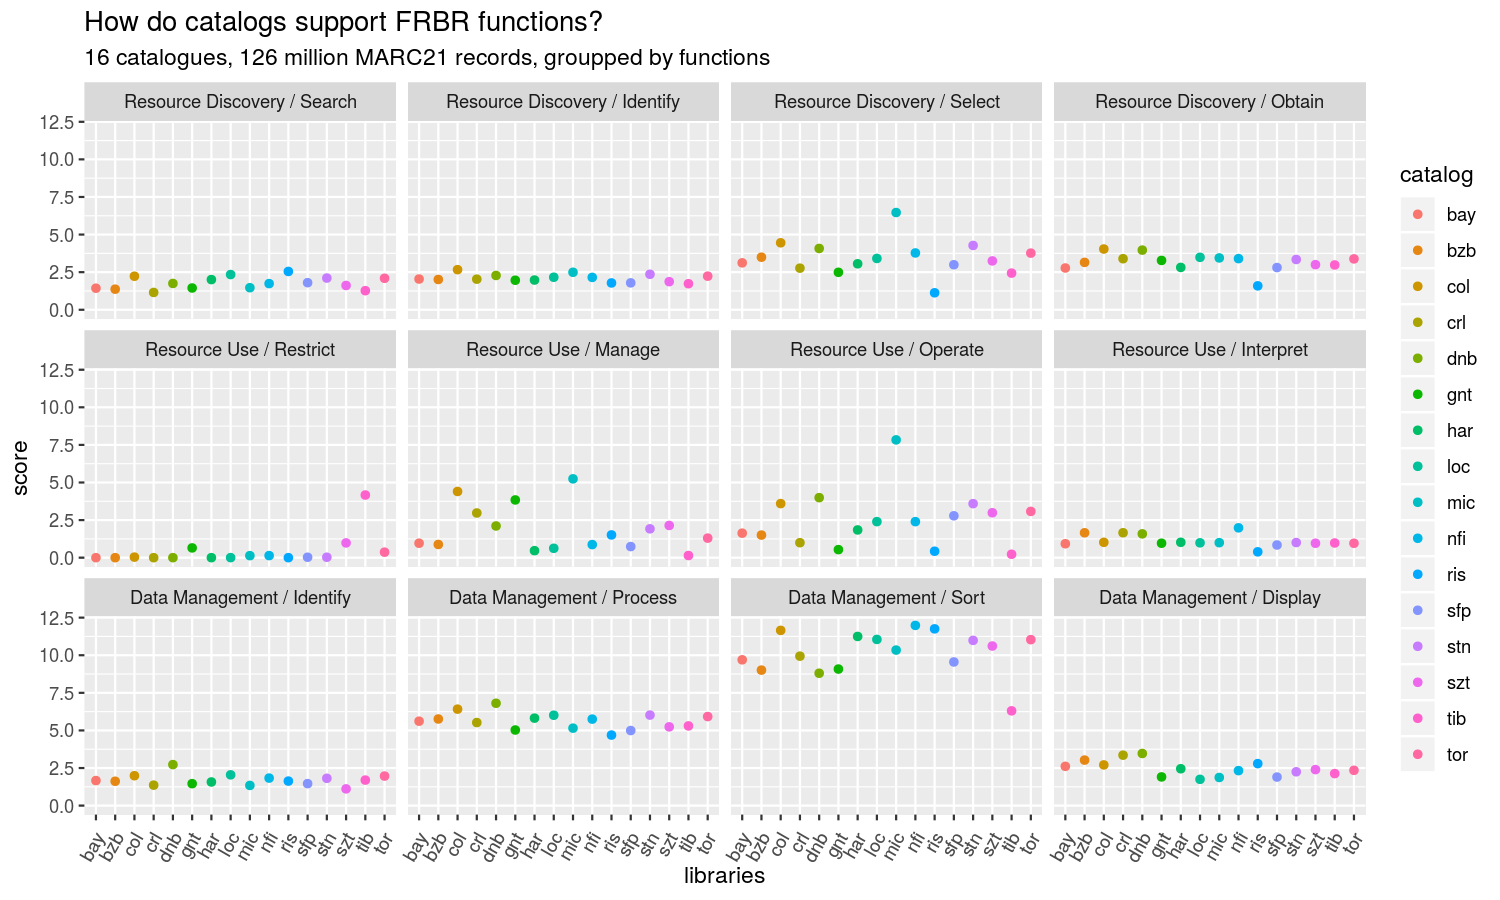
\includegraphics[width=\textwidth]{images/chapter04/functional-analysis-of-catalogs-by-catalogs.png}
\caption{Support of user tasks per catalogs I. Comparison per catalog}
\label{figure:functions-by-catalogs}
\end{figure}

\begin{figure}
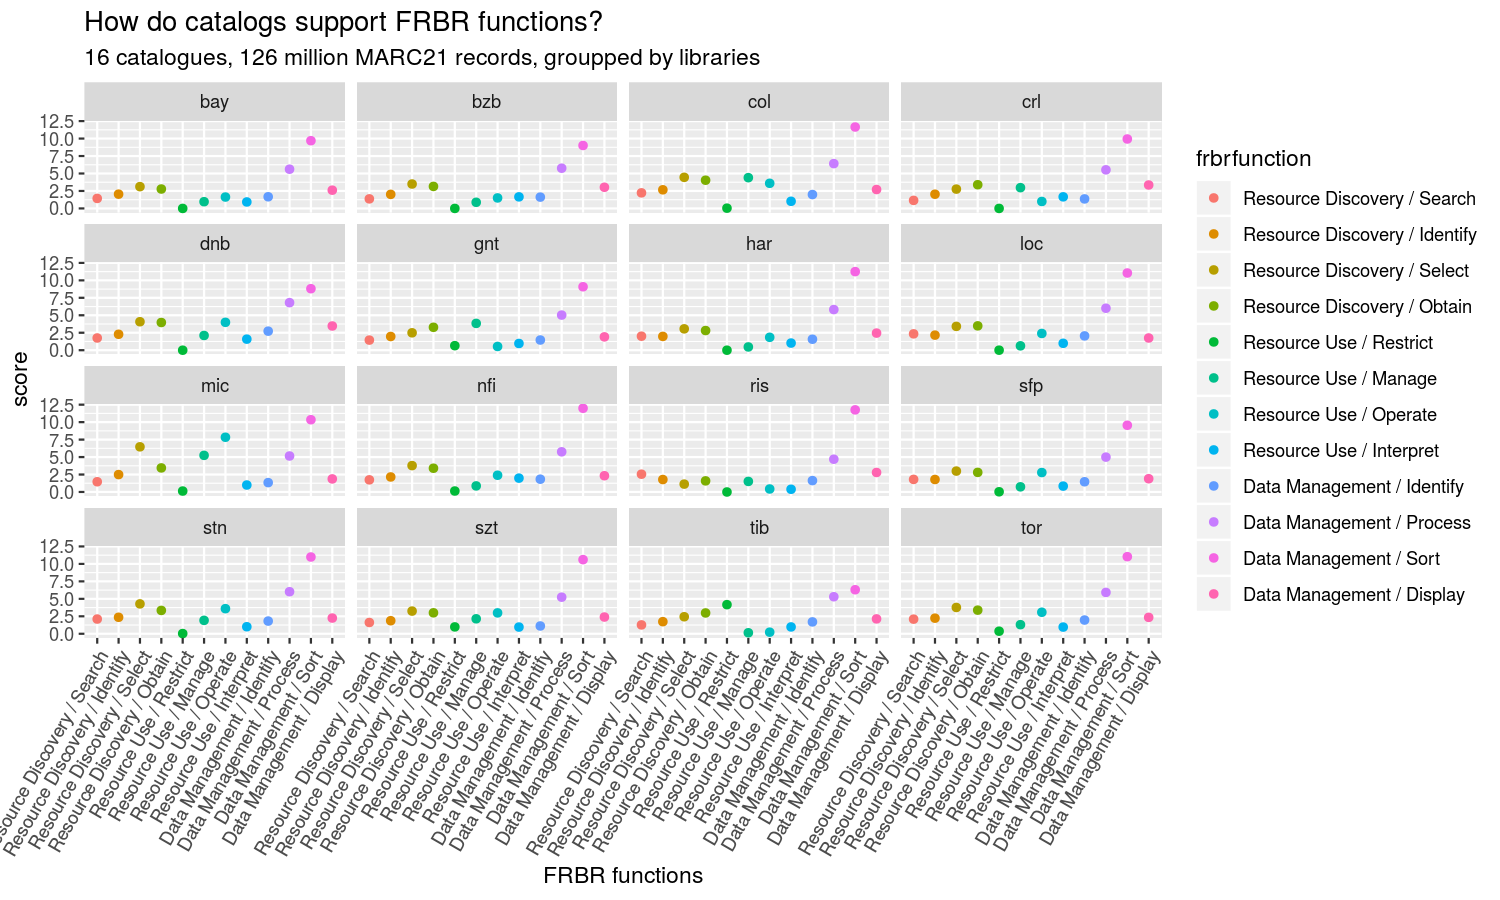
\includegraphics[width=\textwidth]{images/chapter04/functional-analysis-of-catalogs-by-functions.png}
\caption{Support of user tasks per catalogs II. Comparison per function}
\label{figure:functions-by-functions}
\end{figure}

\afterpage{%
    \clearpage% Flush earlier floats (otherwise order might not be correct)
    \thispagestyle{empty}% empty page style (?)
    \begin{landscape}% Landscape page
\begin{table*}
\caption{Support of user tasks (average score, scale: 0-100)}
\label{table:functional-analysis}
\hspace{-1cm}
\begin{minipage}{\columnwidth} %{\columnwidth}
\begin{center}
\begin{tabular}{lrrrrrrrrrrrrrrrr}
\toprule
function & bay & bzb & cer & col & dnb & gen & har & loc & mic & nfi & ris & sfp & sta & szt & tib & tor \\
\midrule
%\midrule
%\midrule
\multicolumn{17}{c}{Resource discovery} \\
%\midrule
Search & 1.4 & 1.4 & 2.2 & 1.2 & 1.7 & 1.4 & 2.0 & 2.3 & 1.5 & 1.7 & 2.5 & 1.8 & 2.1 & 1.6 & 1.3 & 2.1 \\
Identify & 1.6 & 1.5 & 2.3 & 1.8 & 1.7 & 1.7 & 1.7 & 1.9 & 1.4 & 1.8 & 2.0 & 1.6 & 1.9 & 1.5 & 1.3 & 1.8 \\
Select & 2.0 & 2.5 & 4.0 & 2.6 & 2.6 & 2.2 & 3.1 & 3.6 & 2.9 & 3.8 & 1.8 & 3.0 & 3.3 & 2.4 & 1.3 & 3.1 \\
Obtain & 2.1 & 2.3 & 3.4 & 3.0 & 3.1 & 2.9 & 2.3 & 3.1 & 1.8 & 2.9 & 1.9 & 2.4 & 2.5 & 2.3 & 2.3 & 2.7 \\
\multicolumn{17}{c}{Resource use} \\
Restrict & 0.0 & 0.0 & 0.0 & 0.0 & 0.0 & 0.6 & 0.0 & 0.0 & 0.1 & 0.1 & 0.0 & 0.0 & 0.0 & 1.0 & 4.2 & 0.4 \\
Manage & 0.6 & 0.6 & 5.9 & 5.0 & 1.0 & 6.5 & 0.8 & 0.9 & 2.4 & 1.1 & 2.6 & 0.9 & 1.2 & 1.8 & 0.1 & 0.9 \\
Operate & 2.1 & 2.0 & 6.8 & 3.1 & 4.5 & 1.6 & 5.8 & 7.2 & 8.3 & 6.3 & 1.4 & 6.4 & 5.5 & 5.0 & 0.0 & 4.5 \\
Interpret & 0.1 & 0.9 & 0.2 & 0.9 & 0.8 & 0.1 & 0.2 & 0.2 & 0.2 & 1.2 & 0.4 & 0.2 & 0.2 & 0.1 & 0.1 & 0.1 \\
\multicolumn{17}{c}{Data management} \\
Identify & 1.3 & 1.2 & 1.8 & 1.0 & 2.3 & 1.2 & 1.4 & 1.6 & 0.9 & 1.6 & 1.2 & 1.2 & 1.4 & 0.9 & 1.3 & 1.6 \\
Process & 2.0 & 2.2 & 2.8 & 1.9 & 3.2 & 1.6 & 2.2 & 2.4 & 1.6 & 2.2 & 1.9 & 2.0 & 2.4 & 1.7 & 1.7 & 2.3 \\
Sort & 9.7 & 9.0 & 11.7 & 9.9 & 8.8 & 9.1 & 11.3 & 11.1 & 10.3 & 12.0 & 11.8 & 9.6 & 11.0 & 10.6 & 6.3 & 11.0 \\
Display & 2.6 & 3.0 & 2.7 & 3.4 & 3.5 & 1.9 & 2.5 & 1.7 & 1.9 & 2.3 & 2.8 & 1.9 & 2.2 & 2.4 & 2.1 & 2.3 \\
\bottomrule
\end{tabular}
\end{center}
%\bigskip
%\footnotesize
%Note: The numbers in the columns represents the percentage of a given type for all issues in the catalog. Character `--' means that a given type does not occur in the catalog, while `0.0' means a percentage close to zero.
\end{minipage}
\end{table*}
    \end{landscape}
    \clearpage% Flush page
}

% \cite{thompson-traill2017}


\section{Future work}

MARC is an evolving standard, its new rules should be implemented in the newer versions of the software. MARC has a number of strict syntactic rules, but there are also semantic rules, which are not as easy to validate. Content wise there are external rule sets such as the ISBD \cite{isbd}, AACR2 \cite{aacr2} or RDA\footnote{http://rda-rsc.org/content/rda\_faq} which were not explored in this research. I would like to encourage the libraries to publish their local MARC element definitions and to update the software with these rules. A web based user interface with faceted search and data visualization is under construction\footnote{https://github.com/pkiraly/metadata-qa-marc-web}. Data science methods provide us with the possibility of deeper analysis. A Gent catalogue record has the following responsibility statement: ``Herr Seele (tekeningen); Toon Coussement (foto's); Peter Claes, Kris Coremans en Hera Van Sande, vakgroep architectuur en stedenbouw Universiteit Gent (vormgeving).'' The same record lists four authority entries: ``Herr Seele'', ``Coussement, Toon'', ``Claes, Peter'', and ``Van Sande, Hera'' while ``Kris Coremans'' is missing. A comparision of the authority entries and a list extracted by named entity detection would highlight the missing name.

\section{Note about reproducibility}

This research analyzed mostly freely available data sources. The download links, format, and license information of each are provided in section 3.2. The analysis software is an open source tool that is available under the GPL-3.0 license. The binary versions are distributed via Maven Central, a repository for Java libraries. The software is properly documented, and provides helper scripts. Continuous integration (via Travis CI) and automatically generated transparent code coverage reports help to maintain the quality of the software. For every research software project it is a crucial point whether the tool could escape the confines of the laboratory walls. The author is happy to cooperate with libraries to improve the software, and thus the quality of the catalogues. The generated reports behind Table \ref{table:proportion-of-issues} and \ref{table:issue-types} are available as supplemental materials\footnote{https://doi.org/10.25625/AMF8JC}.

\section{Acknowledgement}
Thanks for Johann Rolschewski and Phú for their help in collecting the list of published library catalog, Jakob Voß for the Avram specification and for his help in exporting MARC schema to Avram, Carsten Klee for the MARCspec. I would like to thank the early users of the software, Patrick Hochstenbach (Gent), Osma Suominen and Tuomo Virolainen (FNL), Kokas Károly and Bernátsky László (SZTE), Sören Auer and Berrit Genat (TIB), Shelley Doljack, Darsi L Rueda, and Philip E. Schreur (Stanford), Marian Lefferts (CERL), Alex Jahnke and Maike Kittelmann (SUB) who provided data, suggestions or other kinds of feedback, Justin Christoffersen for language assistance. Special thanks to Reinhold Heuvelmann (DNB) for terminological and language suggestions.

% \bibliographystyle{acm}
% \bibliography{bibliography-for-papers}
